% !TEX root = main.tex
% This is samplepaper.tex, a sample chapter demonstrating the
% LLNCS macro package for Springer Computer Science proceedings;
% Version 2.21 of 2022/01/12
%
\documentclass[runningheads]{llncs}
%
\usepackage[T1]{fontenc}
% T1 fonts will be used to generate the final print and online PDFs,
% so please use T1 fonts in your manuscript whenever possible.
% Other font encondings may result in incorrect characters.
%
\usepackage{graphicx}
\usepackage{float}
\usepackage{booktabs}
\usepackage{siunitx}
% Used for displaying a sample figure. If possible, figure files should
% be included in EPS format.
%
% If you use the hyperref package, please uncomment the following two lines
% to display URLs in blue roman font according to Springer's eBook style:
% \usepackage{color}
%\renewcommand\UrlFont{\color{blue}\rmfamily}
%
\begin{document}
%
\title{Stateless Light Clients for PoS Blockchains}
%
%\titlerunning{Abbreviated paper title}
% If the paper title is too long for the running head, you can set
% an abbreviated paper title here
%
\author{Paul Etscheit}
%
\authorrunning{F. Author et al.}
% First names are abbreviated in the running head.
% If there are more than two authors, 'et al.' is used.
%
\institute{TU Berlin}
%
\maketitle              % typeset the header of the contribution
%
\begin{abstract}
We present a stateless light client design applicable to any Proof-of-Stake blockchain with a deterministic finality gadget. This architecture uses recursive STARKs to compress the chain's validation history into a single, constant-sized proof. By operating exclusively on finalized blocks, its validation logic is deterministic, circumventing the need for stateful fork resolution. State is passed cryptographically between proofs, enabling on-demand verification without persisted data. Our proof-of-concept for Ethereum confirms the design's feasibility, showing that proving costs stabilize at a quasi-constant rate. This method offers a robust solution to weak subjectivity and provides an efficient primitive for blockchain interoperability.

\keywords{Light Clients \and Proof-of-Stake \and Zero-Knowledge Proofs \and STARKs \and Recursion \and Statelessness \and Blockchain Interoperability.}
\end{abstract}
%
%
%
\section{Introduction}
\label{sec:introduction}

The evolution of light client design reveals a persistent trade-off between security, efficiency, and statefulness. Early SPV clients offered a simple model but scaled linearly with chain history \cite{Nakamoto2008Bitcoin}. Subsequent PoW clients achieved sub-linear complexity \cite{Bunz2020FlyClient,Kiayias2020Nipopow}, but these designs are inapplicable to PoS systems. PoS light clients, including those used in IBC, are secure but require clients to track dynamic validator sets, making them inherently stateful and costly to operate on-chain \cite{Goes2020IBC}.

ZK-powered clients such as Plumo reduce the on-chain computational footprint but do not eliminate the need for perpetual state updates \cite{Gabizon2021Plumo}. Mina demonstrated that an entire blockchain's history could be recursively compressed into a single proof, but its internal need to resolve forks makes its client architecture stateful by necessity \cite{Bonneau2020Coda}. A gap therefore exists for a client that combines the recursive efficiency of Mina with a design that achieves true statelessness for verifying an external chain.

This research aims to fill that gap. We propose an architecture for a ZK light client that is:
\begin{itemize}
    \item \textbf{Recursive}, compressing the entire validation history of a PoS blockchain into a single, constant-size proof.
    \item \textbf{Deterministic}, operating exclusively on finalized blocks to circumvent the complexity and state requirements of fork-choice rules.
    \item \textbf{Stateless}, enabling on-demand verification of the chain head without any persisted state, thereby creating a mechanism for on-demand verification.
\end{itemize}

The goal is to demonstrate a light client that can serve as a highly efficient and trustless primitive, applicable to a wide range of applications.

\section{Background}

This section traces the evolution of light client design, from its origins in Proof-of-Work systems to the complex challenges introduced by Proof-of-Stake consensus and the recent advent of zero-knowledge techniques. We examine how each major architectural shift has attempted to balance the competing demands of security, decentralization, and computational efficiency. By understanding this historical progression, we can better contextualize the specific trade-offs addressed by the stateless, recursive architecture proposed in this paper.

\subsection{Historical Roots: SPV and Proof-of-Work}
The first mention of a light client can be found under the name of Simple Payment Verification (SPV) in Bitcoin's whitepaper~\cite{Nakamoto2008Bitcoin}. In a Proof-of-Work (PoW) system, chain validity is determined by the cumulative work of the longest chain, where work is proven by finding a block hash that meets a specific difficulty target. An SPV client leverages this by downloading and verifying only the sequence of block headers. To confirm a specific transaction, a client receives a Merkle proof from a full node, cryptographically verifying the transaction's inclusion in a block whose header is already part of the validated chain.

Subsequent research on PoW light clients focused primarily on reducing this linear bandwidth requirement. Foundational work on Non-Interactive Proofs of Proof-of-Work (NIPoPoWs) first achieved logarithmic ($\mathcal{O}(\log n)$) complexity by using statistically rare "superblocks" to form a skip-list structure over the chain~\cite{Kiayias2020Nipopow}. FlyClient later refined this approach by using Merkle Mountain Range (MMR) commitments, enabling support for variable-difficulty chains while retaining logarithmic costs~\cite{Bunz2020FlyClient}. More recently, Blink introduced an interactive protocol that achieves optimal constant ($\mathcal{O}(1)$) complexity by having a client inject a random challenge into the chain, trading latency for a minimal proof size~\cite{Aumayr2024Blink}.


\subsection{The PoS Era \& Light-Client Complexity}
The shift from PoW to Proof-of-Stake (PoS) consensus breaks the simplicity of SPV clients. In PoS, chain validity is determined not by cumulative computational work, but by signatures from a committee of validators weighted by economic stake. This paradigm introduces several new complexities for light clients~\cite{Chatzigiannis2021SoK}.

First, clients must track the \textit{dynamic validator set}, requiring them to maintain a persistent state of active validators and their voting power. Second, they incur a significant \textit{signature verification load}, as each block may require checking hundreds of signatures. Additionally, PoS clients must contend with \textit{weak subjectivity} to prevent long-range attacks. Unlike in PoW, where the heaviest chain is objectively canonical, a PoS client cannot securely sync from genesis and must instead start from a trusted recent checkpoint.

To manage these challenges, PoS systems have developed specialized mechanisms. Ethereum introduced a sync committee, a smaller, rotating subset of validators designated to sign blocks for light clients, which significantly reduces the signature verification load \cite{Ethereum2025ConsensusSpecs}. Despite these optimizations, the fundamental requirements of statefulness and perpetual syncing persist, as clients must continuously track validator set changes to remain secure.

\subsection{On-chain PoS Light Clients in IBC}
The Inter-Blockchain Communication Protocol (IBC) provides a standardized method for achieving interoperability between sovereign blockchains through on-chain light clients~\cite{Goes2020IBC}. In the IBC model, a smart contract on a destination chain functions as a light client for a source chain. Off-chain relayers feed this on-chain client with headers and signatures from the source chain. By maintaining a validated sequence of these headers, the client can verify state proofs, enabling trustless communication and asset transfers between chains.

While IBC has been widely adopted within the Cosmos ecosystem, where light clients are often implemented as efficient, core modules, its architecture presents significant challenges for broader adoption. Deploying an IBC client as a standard smart contract on a general-purpose chain like Ethereum is prohibitively expensive. These costs arise from two main sources: the perpetual state storage required to track the source chain's validator set, and the high computational (gas) cost of verifying non-native signature schemes on-chain \cite{Goel2022IBCZKSnarks}. The model's reliance on relayers to continuously submit header updates incurs constant transaction fees, making it a stateful and costly system to maintain.

\subsection{ZK-Compressed Light Clients}
A significant evolution in light client design utilizes zero-knowledge (ZK) proofs to compress heavy on-chain computation. The core principle is to outsource computationally intensive tasks, such as batch-verifying validator signatures, to a powerful off-chain prover. This prover generates a succinct ZK proof of the computation's validity. An on-chain smart contract then only needs to verify this proof, significantly reducing the on-chain verification costs.

Pioneering systems demonstrated the viability of this model. Plumo, designed for the Celo blockchain, uses SNARKs to compress updates from a large sync committee into a single proof\cite{Gabizon2021Plumo}. Similarly, Telepathy uses ZK-SNARKs to reduce the cost of verifying Ethereum's sync committee signatures for cross-chain applications\cite{Succinct2023Telepathy}. This concept has been extended to other ecosystems, with proposals to build ZK-based light clients for protocols like IBC\cite{Goel2022IBCZKSnarks,Succinct2025SP1}.

However, while these clients reduce on-chain costs, they introduce new trade-offs. Proof generation, though performed off-chain, can be resource-intensive and add latency to the update process. Additonally, these designs do not eliminate the need for on-chain state. The client contract must still store data such as the latest verified header or validator set commitment. This requires perpetual, stateful updates to keep the client synchronized, incurring costs regardless of whether it is actively being used.

\subsection{Recursive Proofs and Succinct Blockchains}
A powerful technique for data compression is recursive proof composition, where a ZK proof is used to verify a previous ZK proof. The Mina protocol pioneered the application of this concept to create a "succinct blockchain"~\cite{Bonneau2020Coda}. In Mina's architecture, generating a new block also requires creating a ZK proof that attests to the block's validity. Crucially, this proof's circuit also verifies the proof of the preceding block. This creates a chain of nested proofs, allowing the validity of the entire blockchain's history to be compressed into a single, constant-sized proof.

A client needs only to download and verify this single, compact proof to be convinced of the current state's validity. From the state commitment included in this proof, any historical data can be verified via a standard Merkle proof, all without referencing any other on-chain state.

However, this cryptographic succinctness proves only state transition validity, not consensus canonicity. An adversary could create an alternative, valid history and generate a competing proof, thus forking the chain. To resolve this, Mina integrates a Proof-of-Stake consensus mechanism, Ouroboros Samasika~\cite{Badertscher2018Samasika}, which uses a stateful fork-choice rule to determine the canonical chain. This reintroduces a critical dependency: to follow the canonical chain, a client must track consensus-related state, undermining the goal of pure stateless verification.

\subsection{From Succinctness to True Statelessness}
\label{sec:towards_stateless}

The gap between a cryptographically succinct blockchain and a truly stateless client is fork resolution. Even if a proof guarantees the validity of a state transition, a client must still determine if that transition belongs to the canonical chain. This challenge first appears as short-range forks, which arise from routine network latency or benign validator disagreements. A succinct system like Mina, for instance, requires its clients to implement a state-dependent fork-choice rule (Ouroboros Samasika~\cite{Badertscher2018Samasika,Bonneau2020Coda}) to select the correct chain tip from competing valid branches. This dependency on consensus state directly precludes stateless operation.

A distinct but related challenge is the long-range attack, a vulnerability specific to PoS systems where an adversary uses old, compromised validator keys to create a plausible alternative history from genesis. This leads to the problem of \textit{weak subjectivity~\cite{Chatzigiannis2021SoK}}, where a client syncing from far in the past cannot distinguish the legitimate chain from a fraudulent one without external guidance. This vulnerability is why Bonnet et al. formally prove that PoS systems are not inherently stateless, as a new node cannot securely determine the canonical state using only genesis information~\cite{Bonnet2020Stateless}. Consequently, clients must rely on a trusted recent checkpoint, reintroducing a need for external trust and state awareness.

This research resolves the fork-choice dilemma by designing a client that operates exclusively on blocks that have achieved \textit{deterministic finality}. Many PoS protocols feature such a mechanism, where a block is confirmed as irreversible by a supermajority of validators (e.g., after two epochs in Ethereum). Constraining the ZK program to validate only these finalized state transitions circumvents the need for a stateful fork-choice rule, as short-range forks are settled before a block is processed. This design also inherently defends against long-range attacks by creating a non-forgeable, cryptographic certificate of the canonical history, thereby addressing the core vulnerability of weak subjectivity without relying on external trust. The result is a client that achieves \textit{strong statelessness}, in the parlance of Bonnet et al., where verification requires only genesis data and a single, self-contained proof, enabling a truly stateless verification model.

\section{Related Work}
\label{sec:related_work}

Our work builds upon several distinct lines of research in light client design, from early Proof-of-Work models to modern ZK-powered systems. While the background section contextualizes these developments, this section explicitly distinguishes our proposed architecture from prior art by highlighting the key limitations we address.

\subsection{PoW and Stateful PoS Light Clients}
Early light clients for PoW systems, from Bitcoin's SPV~\cite{Nakamoto2008Bitcoin} to sub-linear protocols like NIPoPoWs~\cite{Kiayias2020Nipopow} and FlyClient~\cite{Bunz2020FlyClient}, are fundamentally tied to PoW-specific security assumptions, such as cumulative work, rendering them incompatible with PoS consensus. PoS light clients, such as those standardized by the Inter-Blockchain Communication Protocol (IBC)~\cite{Goes2020IBC}, correctly model PoS security but are inherently stateful. They require an on-chain contract to perpetually store and update the source chain's validator set, incurring continuous maintenance costs and a significant state footprint~\cite{Goel2022IBCZKSnarks}.

Our approach differs by being designed for PoS from the ground up while targeting true statelessness. Instead of tracking validator sets or cumulative work, our client verifies a single, self-contained proof of the chain's evolution up to a finalized state, eliminating the need for persistent on-chain storage and ongoing updates.

\subsection{ZK-Powered Stateful Light Clients}
A recent class of ZK-powered light clients, including Plumo~\cite{Gabizon2021Plumo} and Telepathy~\cite{Succinct2023Telepathy}, effectively reduces on-chain \textit{computation} by verifying large signature sets off-chain. However, they do not compress on-chain \textit{state}. These systems rely on a traditional smart contract model where the contract itself stores a commitment to the latest validator or sync committee. Advancing the client requires a state-modifying transaction that proves a committee handoff and writes the new committee's commitment to the contract's storage. This reliance on an on-chain state anchor intrinsically links proof verification to the host chain, limiting the portability of the verified data to contexts where the contract's state is accessible.

Our architecture replaces this on-chain state storage with cryptographic accumulation within the recursive proof. Instead of a smart contract storing the current validator set commitment, this commitment is encoded as a public output of the latest ZK proof. To process a subsequent block, the prover uses this output commitment as a public input for the next proof, which in turn exposes the next validator set commitment as an output. State is thereby carried forward entirely within the sequence of proofs, never touching persistent on-chain storage. Consequently, the proof chain can be advanced indefinitely off-chain, making on-chain verification a stateless, on-demand transaction. This model eliminates the perpetual synchronization costs required by a stateful contract, which accrue even when the client is not being used.

\subsection{Succinct Blockchains vs. Stateless Clients}
The Mina protocol pioneered the use of recursive proofs to create a "succinct blockchain," compressing the entire transaction history into a constant-sized proof~\cite{Bonneau2020Coda}. While cryptographically succinct, its light client architecture is not stateless. To follow the canonical chain, a client must implement Mina's internal, state-dependent fork-choice rule, Ouroboros Samasika~\cite{Badertscher2018Samasika}.

The crucial differentiation in our work lies in its external perspective and focus on finality. By designing a client for an \textit{external} chain and exclusively proving blocks that have achieved deterministic finality, we circumvent the need for stateful, consensus-level fork-choice logic. This design choice is what allows us to achieve the true statelessness that a client internal to an L1, which must participate in fork resolution, cannot.

\subsection{Stateless and Recursive Clients for Ethereum}
Recent ZK-based light clients for Ethereum, such as Telepathy~\cite{Succinct2023Telepathy} and proofs leveraging SP1~\cite{Succinct2025SP1}, have demonstrated how to significantly reduce on-chain gas costs by compressing sync committee signature verification into a ZK-SNARK. While computationally efficient, these clients remain architecturally stateful. They rely on an on-chain smart contract to store the public keys of the current sync committee. Consequently, advancing the client requires a state-modifying transaction that proves the committee handoff and updates this on-chain storage.

Our work introduces a fundamentally different, recursive architecture to achieve true statelessness. Instead of depending on contract storage, we embed the committee's identity directly into the chain of proofs. Each new proof validates a subsequent time period and, crucially, recursively verifies the STARK proof from the preceding period. This composition allows the current committee's identity to be passed as a public input from the previous proof, while the next committee's identity is exposed as a public output. This creates a cryptographic chain of custody for the state, yielding a client that can validate a continuous history of committee handoffs with a single, self-contained proof. The result is a truly stateless design that eliminates the costs and complexities of perpetual on-chain synchronization.

\section{System Design and Implementation}
\label{section:implementation}
We now detail the design and implementation of our stateless light client. The proposed solution is a minimal implementation focusing on the core logic: sync committee signature verification for each epoch and the state handoff between sync committee terms.

\subsection{Architecture}
The implementation consists of two primary components: an off-chain backend service and a Cairo program. The system is designed to prove the progression of the Ethereum beacon chain on a per-epoch basis, where an epoch represents a 6.4-minute interval (32 slots), generating a new proof for each incremental update.

The \textbf{backend service} acts as an orchestrator. It monitors the Ethereum network for finalized headers and gathers the corresponding sync committee signatures and any required Merkle proofs. It then executes the Cairo program with these inputs to produce an execution trace. This trace is submitted to StarkWare's Shared Prover (SHARP), which generates the STARK proof for the computation. The backend service retrieves the generated proof from SHARP and persists it, making it available for the next recursive step.

The core logic resides in the \textbf{Cairo program} (\texttt{recursive\_update.cairo}), which has two main responsibilities. First, it performs the \textit{epoch validation}: verifying the BLS signatures for a given epoch's header and decommiting the relevant state. Second, it handles the \textit{recursive verification}: it contains an in-circuit STARK verifier that proves the validity of the proof from the preceding epoch. This recursive composition is the key mechanism that allows state to be passed cryptographically between proofs, rather than being stored on-chain, as detailed in the following section.

\begin{figure}
    \centering
    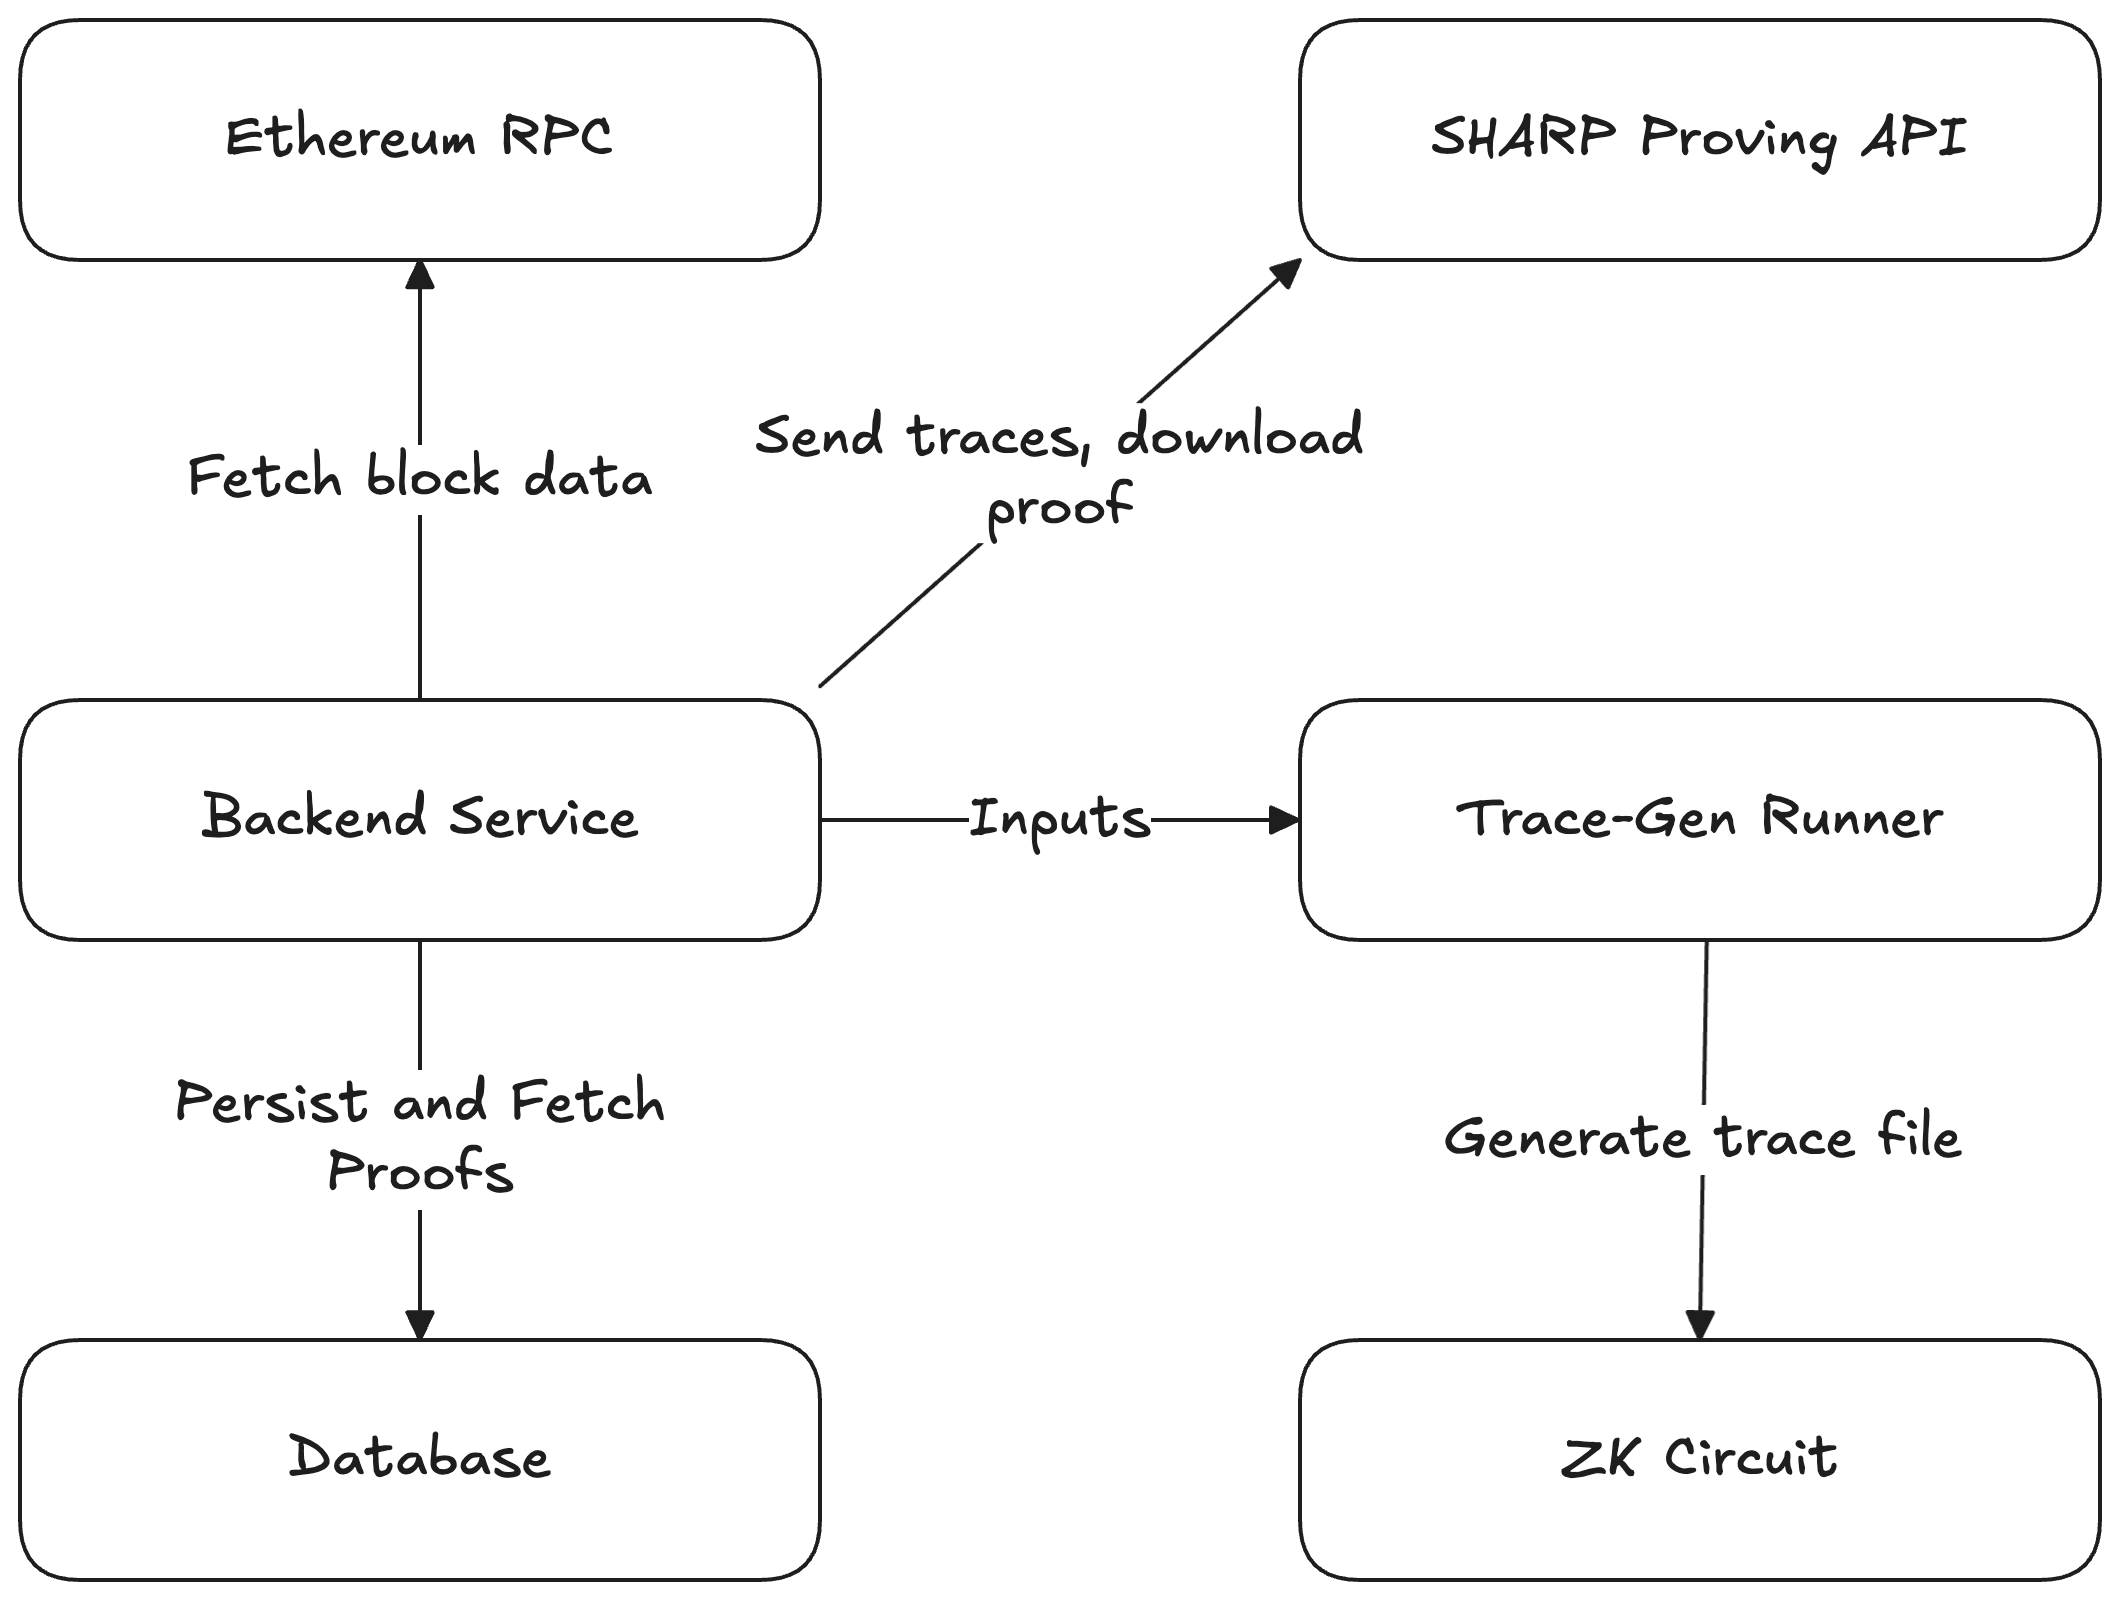
\includegraphics[width=0.8\textwidth]{diagrams/high_level.png}
    \caption{High level system diagram.}
    \label{fig:high_level}
\end{figure}

\subsection{Stateless State Progression via Recursion}
\label{subsection:stateless_recursion}

Our design achieves statelessness by replacing on-chain state storage with a cryptographic state-passing mechanism embedded within the recursive proof sequence. The sole piece of state that must be tracked is the identity of the current sync committee, which we represent as a SHA-256 hash of its aggregate public key, termed the \textit{committee hash}. This hash is passed from one proof to the next, enabling the trustless verification of new headers, which in turn can be used to decommit the next term committee public key. This mechanism allows the system to stay in sync perpetually, without requiring any externally trusted state.

\subsubsection{Recursive State Management}
Before validating the actual signatures, we need to access the sync committees public key of the specific term. As already described above, we can decommit this value from the previous light client update proof output. As the first ever proof has no preceeding proof, we have 2 cases:

\begin{itemize}
    \item \textbf{Genesis Case:} A recursive chain of trust must begin from a secure, immutable anchor. For our system, this is a hardcoded genesis committee hash, corresponding to a finalized sync committee from the target chain's history. When the circuit is run for the first time, it bypasses the recursive verification step. Instead, it directly uses this trusted genesis hash to perform the initial epoch validation via \texttt{run\_epoch\_update}. The resulting proof, $\pi_0$, establishes the first valid state and serves as the foundation for all subsequent proofs in the chain.

    \item \textbf{Recursive Case:} For every subsequent proof, the circuit's primary responsibility is to verify the STARK proof from the immediately preceding step using an in-circuit verifier (\texttt{verify\_cairo\_proof}). After verifying the previous proof, it extracts the committee hash from that proof's public output. This extracted hash is then passed as the trusted input to the Epoch Validation stage for the current period. This step cryptographically ensures that the state from period $i-1$ is correctly used to validate period $i$.
\end{itemize}

\subsubsection{Epoch Validation Logic}
Once the Recursive State Management stage provides a trusted committee hash, the circuit proceeds to validate the new epoch's data against it. This stage executes the core consensus-checking logic.

\begin{itemize}
    \item \textbf{Core Validation (\texttt{run\_epoch\_update}):} The circuit executes three main checks: (1) it reconstructs the beacon header root via its specified SSZ hash structure; (2) it performs a BLS pairing check to verify the sync committee's aggregate signature against the header root, using the committee hash to ensure the signers are correct; and (3) it verifies a Merkle proof for the inclusion of the execution payload header within the beacon state.
    
    \item \textbf{Committee Transition (\texttt{run\_committee\_update}):} A sync committee is in term for 256 epochs (roughly 27 hours), and the subsequent committee's key is available in the beacon state one term in advance. The circuit detects a transition based on the slot number and executes an additional routine to decommit the next committee's public key from the state via a Merkle proof. The hash of this new key is computed and exposed as the \texttt{next\_committee\_hash} in the public output of the proof, ready to be used by the subsequent recursive step.
\end{itemize}

\subsubsection{Circuit Output and Statelessness}
The design's two-stage, recursive structure achieves statelessness by embedding all required state within the public output of each generated proof. This eliminates the need for any persistent on-chain storage for the light client's state. The public output of the circuit is comprised of the following data:

\begin{itemize}
    \item \textbf{Chain Data:} The beacon header root, state root, execution header root, and corresponding block heights. This is the verifiable data that a consuming application would use.
    \item \textbf{Current Committee Hash:} The SHA-256 hash of the committee that validated the \textit{current} epoch. This serves as the primary state input for verifying the \textit{next} proof in the chain.
    \item \textbf{Next Committee Hash:} The SHA-256 hash of the upcoming committee, decommitted from the state. This becomes the active committee hash after a transition period.
\end{itemize}

\begin{figure}[H]
    \centering
    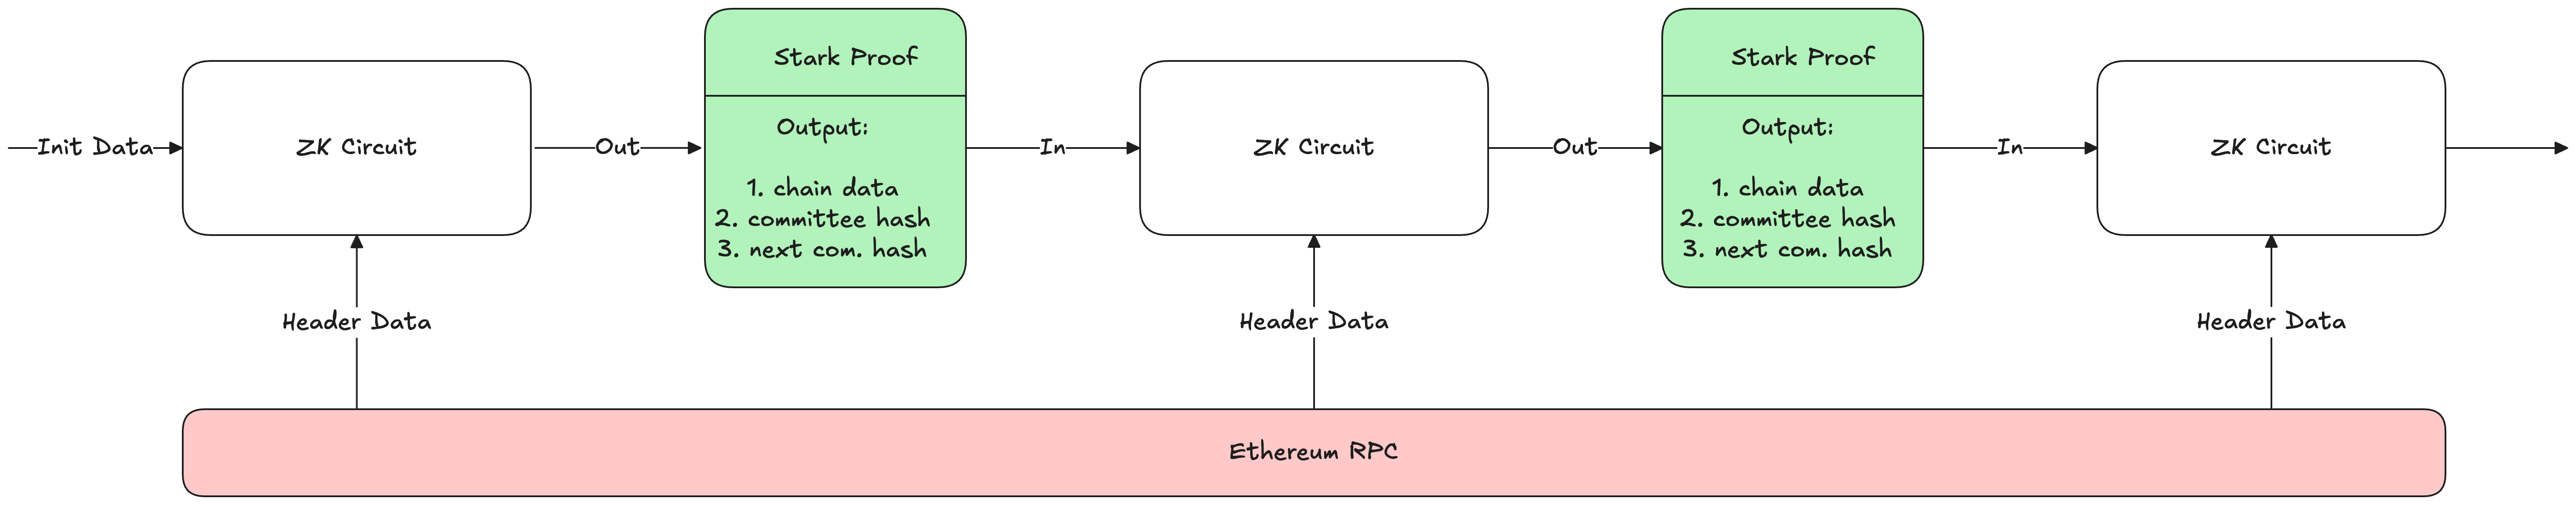
\includegraphics[width=1\textwidth]{diagrams/recursion_diagram.png}
    \caption{Recursive chaining of proofs, passing trusted state between invocations.}
    \label{fig:recursion_diagram}
\end{figure}

As a result, our approach encapsulates the state within the proof itself, making it available for an application to consume, or the next light client update. Verification becomes a pure, `view`-like function call that validates a self-contained proof without reading from or writing to contract storage, thereby achieving a stateless verification model where the trust anchor is the validity of the previous proof, not a mutable storage slot.

\subsection{Development Stack}
\label{subsection:development-stack}
The implementation utilizes the Cairo stack. The core components of our development and execution stack are as follows:

\begin{itemize}
    \item \textbf{Language and Toolchain:} The circuit is implemented in Cairo v0.13.5 (also known as Cairo Zero). We use the corresponding \texttt{cairo-lang} toolchain for compilation and a Rust-based Cairo VM for generating execution traces locally.
    \item \textbf{Cryptographic Libraries:} To implement cryptographic primitives efficiently, we leverage the Garaga~\cite{Prime2025Garaga} and Garaga Zero libraries. These provide optimized circuits for operations like BLS pairing checks by utilizing Cairo's native \texttt{modulo} builtin, which is critical for performance.
    \item \textbf{Prover:} Proof generation is handled by StarkWare's Shared Prover (SHARP), which provides a production-grade service for generating STARK proofs from valid execution traces.
\end{itemize}


\subsection{Implementation and Technical Challenges}
Several technical challenges were addressed during implementation, primarily related to the computational cost of cryptographic primitives within the Cairo VM.
\begin{itemize}
    \item \textbf{Hash-to-Curve Algorithm:} The hash-to-curve function, a prerequisite for BLS signature verification, is complex to implement. Performing this operation in Cairo is particularly expensive due to the overhead of emulating non-native field arithmetic. To mitigate this, we utilized the Garaga library~\cite{Prime2025Garaga}, which provides highly optimized circuits for cryptographic operations by directly leveraging Cairo's `modulo` builtin, thereby avoiding costly emulation.

    \item \textbf{BLS Pairing Check:} The final pairing check in the BLS verification scheme is another performance-critical component. As with hash-to-curve, a naive implementation incurs significant costs from field emulation. We again employed the Garaga library~\cite{Prime2025Garaga} for an efficient implementation that dramatically reduces the computational footprint of the pairing operation.
    
    \item \textbf{STARK Recursion Cost:} A core design trade-off is the cost of in-circuit STARK verification. While STARKs provide transparency (no trusted setup) and conjectured post-quantum security, verifying a STARK proof is more computationally intensive than verifying common elliptic-curve-based SNARKs (e.g., Groth16). This cost is a primary driver of overall prover time in our recursive architecture.
\end{itemize}

\subsection{Implementation Scope and Limitations}
The current implementation serves as a proof-of-concept to demonstrate the computational feasibility of our proposed stateless, recursive architecture. In this section, we outline the primary limitations of the system in its current form. These include both inherent architectural boundaries, such as its reliance on the sync committee protocol, and deliberate simplifications made to create a focused benchmarking environment for the core cryptographic components.

\begin{itemize}
    \item \textbf{Reliance on Sync Committee Consensus:} Our client's logic is based on Ethereum's sync committee protocol, not the full Gasper (Casper-FFG and LMD-GHOST) consensus rules that a full node validates. While the sync committee is a native and secure consensus gadget designed for light clients, this means our proof attests to the validity of the light client protocol's view of the chain, rather than verifying the entire consensus mechanism.

    \item \textbf{Lack of Historical Data Commitment:} The current circuit validates the progression of the chain head but does not commit the history of verified headers to a cryptographic accumulator like a Merkle Mountain Range. While the latest proof attests to the current head, it cannot be used to efficiently decommit historical data. Integrating such a structure would be necessary for a full-featured client but would increase proving costs due to the additional hashing. The impact of this will be explored in future research.
    
    \item \textbf{Simplified Fork Handling:} The implementation does not include logic to handle chain reorganizations (forks). Implementing fork resolution is not expected to generate a large amount of additional constraints, but does require the availibility of historical headers. As these are not available, the fork resolution was not implemented.

    \item \textbf{Omission of Circuit Integrity Checks:} Two important constraints are not enforced in the implementation, resulting in a more flexible benchmarking setup. For one, we do not enforce a gap-free recursion, which enables us to skip epochs for benchmarking. Additionally, we dont enforce the same program is used for each recursive step, which enables us to fix smaller bugs in the implementation, which would otherwise require starting the entire benchmark from genesis again. 
\end{itemize}

\section{Evaluation}
\label{section:evaluation}

In this section, we evaluate the performance of our stateless, recursive light client. The primary goal is to demonstrate the computational feasibility of the architecture and establish a performance baseline. We measure performance using two key metrics: (1) the number of Cairo VM steps, which serves as a proxy for computational cost, and (2) the wall-clock proving time, reported by StarkWare's SHARP prover. Our analysis is structured to first isolate the cost of recursion itself, then measure the complexity of the full light client circuit, and finally examine real-world proof generation times.

\subsection{Experimental Setup}
\label{subsection:experimental-setup}
We evaluated our implementation using the following setup:

\begin{itemize}
    \item \textbf{System Components}: An off-chain coordinator, running on an Apple M1 Pro (32GB RAM), fetches data from an Ethereum RPC endpoint and generates the execution trace. Proof generation is delegated to StarkWare's Shared Prover (SHARP) via the Atlantic Proving Service API, as local proving is not feasible. The SHAPR proving API utilizes the open source Stone Prover \cite{StarkWare2023Stone}.

    \item \textbf{Test Scenarios}: Our evaluation comprises two distinct experiments.
        \begin{itemize}
            \item \textbf{Recursive Counter}: To establish a baseline for the cost of recursion, we first evaluated a minimal recursive program that only increments a counter.
            \item \textbf{Light Client Circuit}: We then recursively proved epochs from Ethereum's Sepolia testnet using our full light client circuit. To efficiently measure the cost of standard updates and periodic committee handoffs, the experiment spanned epochs 248576 to 249504, sampling one epoch at a 32-epoch interval.
        \end{itemize}

    \item \textbf{Metrics}: Performance is measured by two key indicators: (1) \textbf{Proving Time}, the wall-clock time reported by the SHARP service for proof generation, and (2) \textbf{Cairo Steps}, the number of virtual machine execution steps, which is a direct proxy for computational cost.
\end{itemize}

\subsection{Evaluation Results}
\label{subsection:evaluation-results}
Following the experimental setup, we now present the quantitative results of our evaluation. The analysis begins by establishing a baseline for the cost of STARK recursion, then examines the computational complexity of the full light client circuit, and finally examines real-world proof generation times.

\subsubsection{Baseline Cost of STARK Recursion}
A large part of the system's computational cost comes from the recursion step. The cost of verifying a STARK proof is not fixed; it depends on the complexity of the program being proven. We can model the cost of the n-th recursive proof, measured in Cairo steps \(S_n\), with the approximation \(S_n \approx C + \alpha \ln S_{n-1}\). Here, \(C\) is the verifier's large, fixed overhead, and \(\alpha\) is a scaling factor sensitive to the proof's trace structure. While verification cost grows logarithmically with trace length (\(S_{n-1}\)), it grows approximately linearly with trace width.

To empirically derive \(C\), we designed a minimal recursive counter program whose own logic is trivial (11 steps). The raw data for this experiment is available in the Appendix (Table~\ref{tab:raw_benchmark_data}). The first recursive step (Round 2) costs 2,322,005 steps. Since the inner program's own cost is negligible, this value provides a direct and strong approximation for the constant overhead: \(C \approx 2.32M\) steps.

\begin{figure}[H]
    \centering
    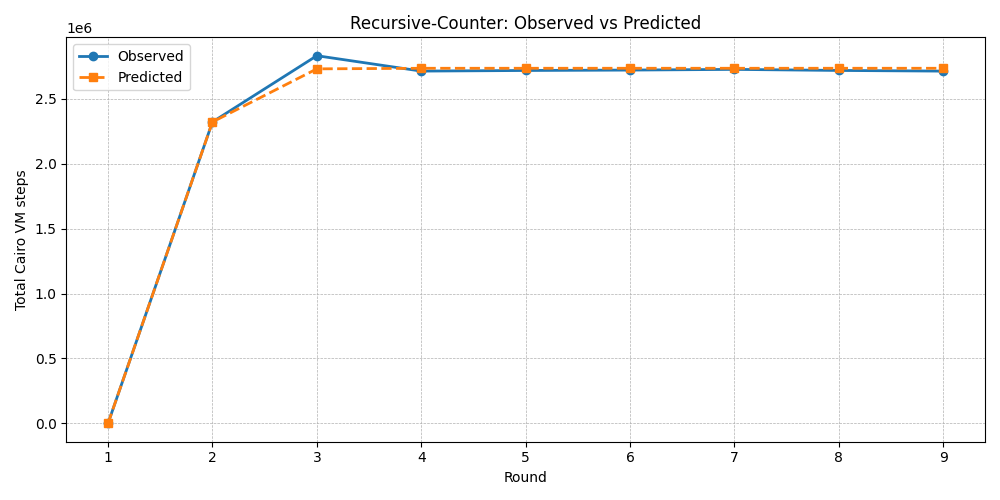
\includegraphics[width=0.8\textwidth]{diagrams/recursive_counter_observed_vs_predicted.png}
    \caption{Observed vs. predicted step counts for a recursive counter. The model (\(S_n \approx 2.32M + 27.9k \ln S_{n-1}\)) shows high accuracy, with predictions for rounds 4-9 falling within 1.1\% of measured values, confirming the logarithmic growth of recursive proving costs.}
    \label{fig:counter_prediction}
\end{figure}

With \(C\) established, we can derive \(\alpha\). This factor is influenced by the program's "layout" (the builtins used), which determines the trace width. For our simple counter, which has a minimal layout and thus a narrow trace, we expect a relatively small \(\alpha\). A least-squares fit on the deeper recursion levels (Rounds 3-9) from our data confirms this, yielding \(\alpha \approx 27,924\). The complete model shows high predictive accuracy, as illustrated in Figure~\ref{fig:counter_prediction}. This analysis confirms that STARK recursion has a large but predictable cost structure, providing an essential baseline for evaluating our main light client circuit, which will have a wider trace and thus a different \(\alpha\).


\subsubsection{Light Client Circuit Steps}
We next analyze the computational cost of the full light client circuit. While this circuit also uses the dynamic layout, its higher use of builtins results in a wider program trace. As predicted by our model, this yields a larger scaling factor, which we empirically derive as \(\alpha \approx 100,327\) using our established baseline for \(C\). The resulting model provides a strong predictive fit, with one notable exception. The anomaly first seen in the baseline experiment reappears: at the third recursive step, the step count unexpectedly plateaus instead of increasing in line with the complexity of the inner proof (\(S_2\)). As this artifact occurs in both experiments, it strongly suggests an intrinsic property or optimization of the in-circuit verifier itself, rather than a facet of our light client logic.

\begin{figure}[H]
    \centering
    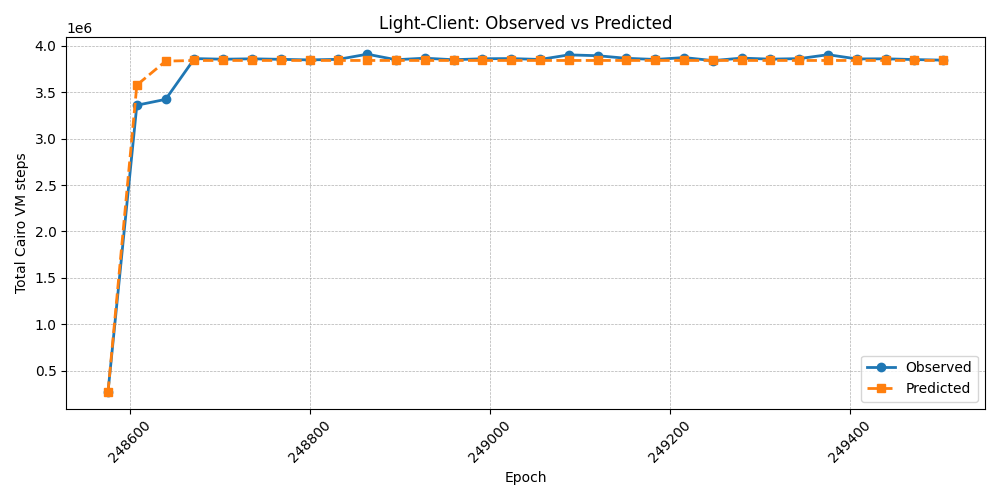
\includegraphics[width=0.8\textwidth]{diagrams/light_client_observed_vs_predicted.png}
    \caption{Observed vs. predicted step counts for a recursive counter. The model (\(S_n \approx 2.32M + 100.33k \ln S_{n-1}\)) shows an accurate approximation}
    \label{fig:light_client_prediction}
\end{figure}

Examining the circuit's performance over 29 recursive invocations reveals a critical property of the architecture. As shown in Figure~\ref{fig:light_client_steps}, the computational cost stabilizes after an initial ramp-up period of approximately four invocations. This finding is significant as it addresses a concern regarding a potential cost feedback loop where each successive proof would slowly become more expensive, gradually accumilating steps. Our results show that the system does not suffer from such unbounded growth. The observed fluctuations in step count are not arbitrary but correspond to predictable, periodic work: the increased cost of sync committee decommitment, which occur roughly every eighth invocation in our test. The system therefore achieves a quasi-constant proving cost, confirming its long-term computational stability.

\begin{figure}[H]
    \centering
    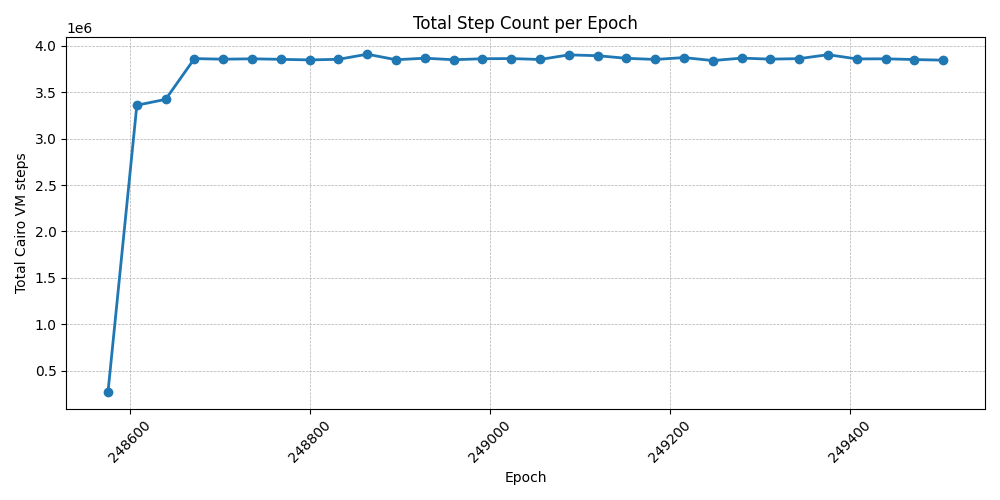
\includegraphics[width=0.8\textwidth]{diagrams/step_count_vs_epoch.png}
    \caption{Measured steps for a given Epoch}
    \label{fig:light_client_steps}
\end{figure}

\subsubsection{Proof Generation Time}
Beyond the abstract cost of Cairo steps, we measured the real-world performance by submitting execution traces to StarkWare's SHARP prover. As shown in Figure~\ref{fig:proving_time}, the wall-clock proving time is largely stable and correlates with the number of Cairo steps. However, the measurements exhibit two significant outliers where the proving time was substantially longer without a corresponding increase in computational complexity. We attribute these anomalies to external factors within the shared proving service, such as variable queue times or infrastructure state, rather than the circuit's intrinsic performance.

The distribution of proving times, also shown in Figure~\ref{fig:proving_time}, confirms this assessment. The majority of proofs were generated within a consistent and predictable time frame, demonstrating the viability of the system despite the occasional latency from the shared infrastructure. This suggests that with a dedicated or more optimized prover, the proving time would be highly consistent.

\begin{figure}[H]
    \centering
    \begin{minipage}{0.48\textwidth}
        \centering
        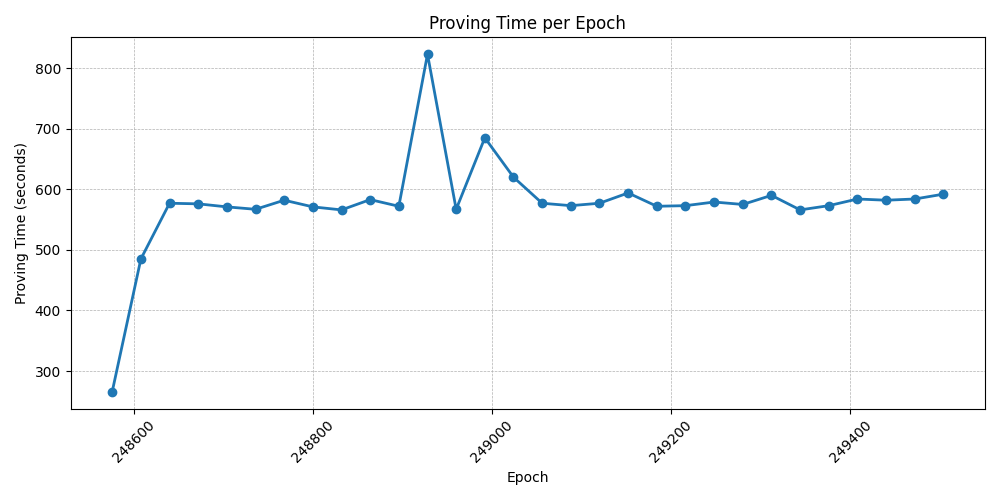
\includegraphics[width=\textwidth]{diagrams/proving_time_vs_epoch.png}
    \end{minipage}\hfill
    \begin{minipage}{0.48\textwidth}
        \centering
        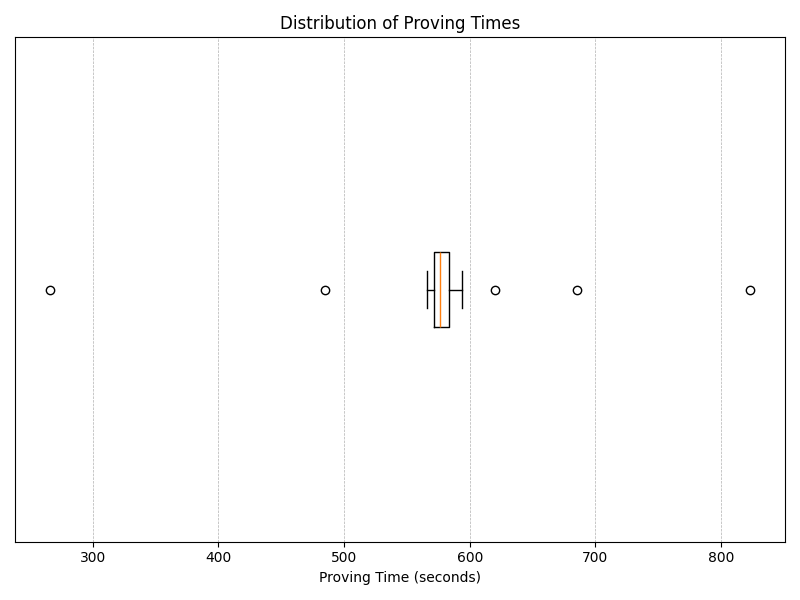
\includegraphics[width=\textwidth]{diagrams/proving_time_distribution.png}
    \end{minipage}
    \caption{Proving time per epoch (left) and its distribution (right). While mostly stable, two outliers suggest variability in the shared proving service.}
    \label{fig:proving_time}
\end{figure}

\subsection{Discussion of Results}
\label{subsection:discussion-of-results}
Our evaluation provides strong evidence for the viability of the proposed architecture and highlights key areas for future optimization.

\begin{itemize}
    \item \textbf{Strengths}: The results successfully demonstrate that the core concept of a stateless, recursive light client is feasible. We show that it is possible to perpetually sync with a PoS chain, accumulating its state transitions into a single, quasi constant-sized ZK proof that enables trustless verification without any external state. A key enabler is the efficiency of the underlying cryptography; using the Garaga library with Cairo's native `modulo` builtin, the entire BLS signature verification process, including hash-to-curve, pairing checks, and signer aggregation, required only approximately 71,000 Cairo steps, or about 5\% of the total computational workload. Furthermore, while STARKs are often considered less efficient for recursion than other proof systems, our findings indicate that the approach is practical even with the original Stone prover (c. 2020), suggesting significant potential for performance gains with more modern provers.

    \item \textbf{Limitations}: The primary trade-off in our design is the cost of recursion itself. As noted, verifying a STARK proof in-circuit is computationally demanding. A critical consideration for future work is how the cost scales as the base circuit grows. Adding features essential for a production client, such as a historical header commitment (e.g., an MMR), would increase the number of constraints in the epoch-validation circuit. This, in turn, increases the complexity and cost of the in-circuit verifier, making every subsequent recursive step more expensive. Quantifying this overhead is essential for understanding the practical limits of the architecture.

    \item \textbf{Robustness}: The fundamental architecture is not specific to Ethereum. Its core principles—verifying finalized state transitions and passing committee commitments via recursion—are generalizable to other PoS blockchains that feature a finality gadget. The demonstrated efficiency of the BLS verification logic makes this approach particularly applicable to the growing number of chains that use BLS-based consensus.
\end{itemize}

\section{Conclusion and Future Work}
\label{section:conclusion}
In this paper, we presented and evaluated a stateless, recursive ZK light client for PoS blockchains. Our evaluation demonstrates the architecture's computational viability, establishing that a perpetual sequence of state transitions can be compressed into a single, quasi constant-sized STARK proof. The average proving time of approximately 9.5 minutes per epoch, using a five-year-old prover, confirms the system is viable, although it is not yet fast enough to keep pace with Ethereum's 6.4-minute epoch time. A production system could manage this latency by strategically generating proofs for every \(k\)-th epoch.

However, a significant architectural challenge remains. The current design only validates the chain head. Extending it to include a cryptographic accumulator, such as a Merkle Mountain Range to commit to historical headers, would increase the base circuit's complexity. This, in turn, would raise the cost of in-circuit STARK verification, making every recursive step more expensive. Quantifying this overhead is a critical area for future investigation. These performance considerations frame the most immediate avenues for future work:

\begin{itemize}
    \item \textbf{Prover Upgrade:} A primary focus is migrating to next-generation provers. Preliminary tests with StarkWare's S-Two prover~\cite{StarkWare2025STwo}, which is based on Circle STARKs~\cite{Habock2024CircleSTARKs}, are highly promising. A non-recursive epoch proof that takes 266 seconds on the production SHARP service can be generated in approximately 13 seconds on a consumer M4 Max laptop. However, realizing these gains in a recursive context is currently infeasible due to the inefficiency of the available in-circuit verifier for Circle STARK proofs.
    
    \item \textbf{Historical Data Accumulation:} Once an efficient recursive verifier is developed, the circuit can be extended to include a cryptographic accumulator, such as a Merkle Mountain Range. This would commit to the entire history of verified headers within the proof itself, transforming the client into a fully succinct verifier for both state and history.
\end{itemize}

\section*{Author's Note}
The author acknowledges the use of large language models (LLMs) to assist in the preparation of this manuscript. These tools were used for specific tasks, including literature review, proofreading for spelling and grammar, and rephrasing to improve clarity. The conceptual framework, technical implementation, experimental results, and all conclusions presented are the original work of the author.


% ---- Appendix ----
\appendix
\section{Benchmark Data}
\label{sec:appendix_benchmark}

\begin{table}[H]
  \centering
  \sisetup{group-separator = {,}}
  \begin{tabular}{lr@{\hspace{2em}} S[table-format=6] @{\hspace{1em}} S[table-format=7,group-separator={,}] @{\hspace{1em}} S[table-format=3]}
    \toprule
    \multicolumn{2}{c}{\textbf{Recursive Counter}} & \multicolumn{3}{c}{\textbf{Light Client Circuit}} \\
    \cmidrule(r){1-2} \cmidrule(l){3-5}
    {Round} & {Steps} & {Epoch} & {n\_steps} & {Proving time (s)} \\
    \midrule
    1  & 11 & 248576 & 273095  & 266 \\
    2  & 2\,322\,005 & 248608 & 3360672 & 485 \\
    3  & 2\,832\,636 & 248640 & 3423795 & 577 \\
    4  & 2\,714\,132 & 248672 & 3863454 & 576 \\
    5  & 2\,718\,837 & 248704 & 3856710 & 571 \\
    6  & 2\,721\,987 & 248736 & 3861068 & 567 \\
    7  & 2\,727\,275 & 248768 & 3855310 & 582 \\
    8  & 2\,719\,123 & 248800 & 3849179 & 571 \\
    9  & 2\,713\,958 & 248832 & 3855476 & 566 \\
    \multicolumn{2}{c}{} & 248864 & 3910611 & 583 \\
    \multicolumn{2}{c}{} & 248896 & 3851028 & 572 \\
    \multicolumn{2}{c}{} & 248928 & 3867636 & 823 \\
    \multicolumn{2}{c}{} & 248960 & 3851033 & 567 \\
    \multicolumn{2}{c}{} & 248992 & 3861700 & 685 \\
    \multicolumn{2}{c}{} & 249024 & 3863629 & 620 \\
    \multicolumn{2}{c}{} & 249056 & 3853890 & 577 \\
    \multicolumn{2}{c}{} & 249088 & 3903427 & 573 \\
    \multicolumn{2}{c}{} & 249120 & 3894427 & 577 \\
    \multicolumn{2}{c}{} & 249152 & 3866374 & 594 \\
    \multicolumn{2}{c}{} & 249184 & 3854135 & 572 \\
    \multicolumn{2}{c}{} & 249216 & 3874342 & 573 \\
    \multicolumn{2}{c}{} & 249248 & 3842016 & 579 \\
    \multicolumn{2}{c}{} & 249280 & 3868387 & 575 \\
    \multicolumn{2}{c}{} & 249312 & 3857436 & 590 \\
    \multicolumn{2}{c}{} & 249344 & 3863031 & 566 \\
    \multicolumn{2}{c}{} & 249376 & 3905394 & 573 \\
    \multicolumn{2}{c}{} & 249408 & 3859813 & 584 \\
    \multicolumn{2}{c}{} & 249440 & 3861020 & 582 \\
    \multicolumn{2}{c}{} & 249472 & 3852910 & 584 \\
    \multicolumn{2}{c}{} & 249504 & 3846529 & 592 \\
    \bottomrule
  \end{tabular}
  \caption{Raw benchmark data for the recursive counter and light client circuits. Measurements taken on 18 July 2025.}
  \label{tab:raw_benchmark_data}
\end{table}

% ---- Bibliography ----
%
% BibTeX users should specify bibliography style 'splncs04'.
% References will then be sorted and formatted in the correct style.
\bibliographystyle{splncs04}
\bibliography{references}


\end{document}